\chapter{軌道計算とDSMC法の連成解析}
\label{chap:couple}

第~\ref{chap:min-knud}章で得られた結果より,
軌道計算で用いられるDKRモデルによる淀み点熱流束と,
DSMC法によって得られる淀み点熱流束が大きく異なることが分かった.
これはDKRモデルは連続体を仮定しており,希薄流で適用することが困難であることを意味する.
従って,自由分子流ではDKRモデルと解離し,連続流に近づくにつれてDKRモデルに一致することが予想される.

本章では,軌道計算における複数地点でDSMC法による流れ場解析を行い,
軌道上でどのように淀み点熱流束が変化するかを調査する.
また,その結果をもとにしてDKRモデルでの淀み点熱流束を補正し,
DSMC法との連成解析として改めて軌道計算を行う.

\section{連成解析の手順}
軌道計算の時間刻み幅は\SI{1e-2}{s}である一方で,
DSMC法の時間刻み幅は\SI{1e-8}{s}から\SI{1e-6}{s}程度であり,
時間スケールが大きく異なる.
従って,連成解析を行うにあたりその手順を工夫する必要がある.

本研究では,Knudsen数と淀み点熱流束に相関があると仮定して,
Knudsen数のオーダーが切り替わるタイミングでDSMC法による流体場解析を行い,
それぞれで淀み点熱流束の補正を行う.
従って,具体的な手順は以下のようになる.
\begin{enumerate}
    \item 初期高度でDSMC法を行う.
    \item DSMC法による結果より淀み点熱流束の補正係数を算出する.
    \item 補正係数を考慮した軌道計算を,Knudsen数のオーダーが切り替わるまで行う.
    \item Knudsen数のオーダーが切り替わる地点の条件を用いてDSMC法による流体場解析を行う.
    \item 以降,手順2から4を流星源が消滅するまで繰り返す.
\end{enumerate}
また,Hendersonによる抗力係数モデル~\cite{henderson1976drag}の妥当性も同様の手順により検証を行う.

\section{抗力係数の補正}
\subsection{DSMC法との連成解析による補正係数の算出}
まず,Hendersonによる抗力係数モデル~\cite{henderson1976drag}の妥当性を検証する.
DSMC法と軌道計算の連成解析によって得られたKnudsen数に対する抗力係数の補正係数を以下の表に示す.
\begin{table}[H]
\centering
\caption{軌道計算およびDSMC法の連成解析による抗力係数の補正係数}
\begin{tabular}{l|cc}
\hline\hline
$Kn$ & 補正係数($C_\mathrm{d}^*$) \\ \hline
\num{1.2d7} & \num{0.908}   \\
\num{1d6  } & \num{0.905}   \\
\num{1d5  } & \num{0.888}   \\
\num{1d4  } & \num{0.935}   \\
\num{1d3  } & \num{1.02  }  \\
\num{1d2  } & \num{0.894}   \\
\num{1d1  } & \num{1.03d0  }\\
\num{2d0  } & \num{1.05}    \\
\num{1d0  } & \num{1.08  }  \\
\num{5d-1} & \num{1.13  }  \\
\num{2d-1 } & \num{1.07 }   \\
\num{1d-1 } & \num{1.03 }   \\ \hline\hline
\end{tabular}
\end{table}
ここで,抗力係数の補正係数は,DSMC法によって得られた抗力係数と,Hendersonによるモデル式で得られた抗力係数の比となっている.
従って,抗力係数の補正係数$C_\mathrm{d}^*$は以下のように与える.
\begin{equation}
    C_\mathrm{d}^* = \dfrac{C_\mathrm{d,DSMC}}{C_\mathrm{d,Henderson}}.
\end{equation}
ただし,$C_\mathrm{d,DSMC},\ C_\mathrm{d,Henderson}$はそれぞれDSMC法で得られた抗力係数とHendersonのモデル式による抗力係数である.

結果を見ると,$Kn = \num{1d7},\ \num{5d-1}$を除いて
$\pm$10\%以下の差異となっており,両者は概ね一致している.

\subsection{補正された抗力係数による軌道への影響}
次に,この補正係数を組み込んだ軌道計算を実施し,補正なしの軌道計算結果と比較する.
補正係数の変化する幅が小さいことから,線形補間などは行わず,ステップ状に補正係数を抗力係数にかけ合わせた.
まず,抗力係数への補正あり・なしの抗力係数変化を図~\ref{fig:couble-cd-cd}に示す.
補正係数をかけた方は高度によってステップ状に抗力係数が変化していることが確認できる.
また,抗力係数への補正あり・なしの流星源速度変化を図~\ref{fig:couble-cd-velo}に示す.
両者は良好に一致しているが,消滅によって途切れるタイミングが補正ありの方が遅くなっていることが分かる.

次に,抗力係数への補正係数あり・なしの質量変化・Reynolds数変化・Knudsen数変化をそれぞれ
図~\ref{fig:couble-cd-mass}から~\ref{fig:couble-cd-kn}に示す.
どの結果においても,補正ありとなしでは良好に一致していることが確認できる.
ただし,速度変化と同様に,消滅のタイミングに差異が生じている.

流星源消滅のタイミングが変化した原因としては,熱流束の見積もりの差異が影響したためと考えられる.
補正あり・なしの流星源が受ける熱流束変化を図~\ref{fig:couble-cd-heat}に示す.
高度80~km付近における熱流束の極大値を見ると,
補正ありの最大熱流束が補正なしのものと比べて小さくなっている.
これによって,アブレーションによる質量減少が遅れ,結果として消滅のタイミングに差異を及ぼしたと考えられる.
しかし,消滅した高度を比較すると,
補正ありの場合で高度67.2~km,補正なしでは高度67.7~kmであり,その差は0.5~kmに留まった.

DSMC法との連成計算による補正を加えた場合とHendersonのモデル式~\cite{henderson1976drag}は
概ね一致した.
すなわち,人工流れ星の軌道上での抗力係数はHendersonのモデル式~\cite{henderson1976drag}に従い,DSMC法との連成計算による補正の必要は無いことが分かった.
\begin{figure}[H]
    \centering
    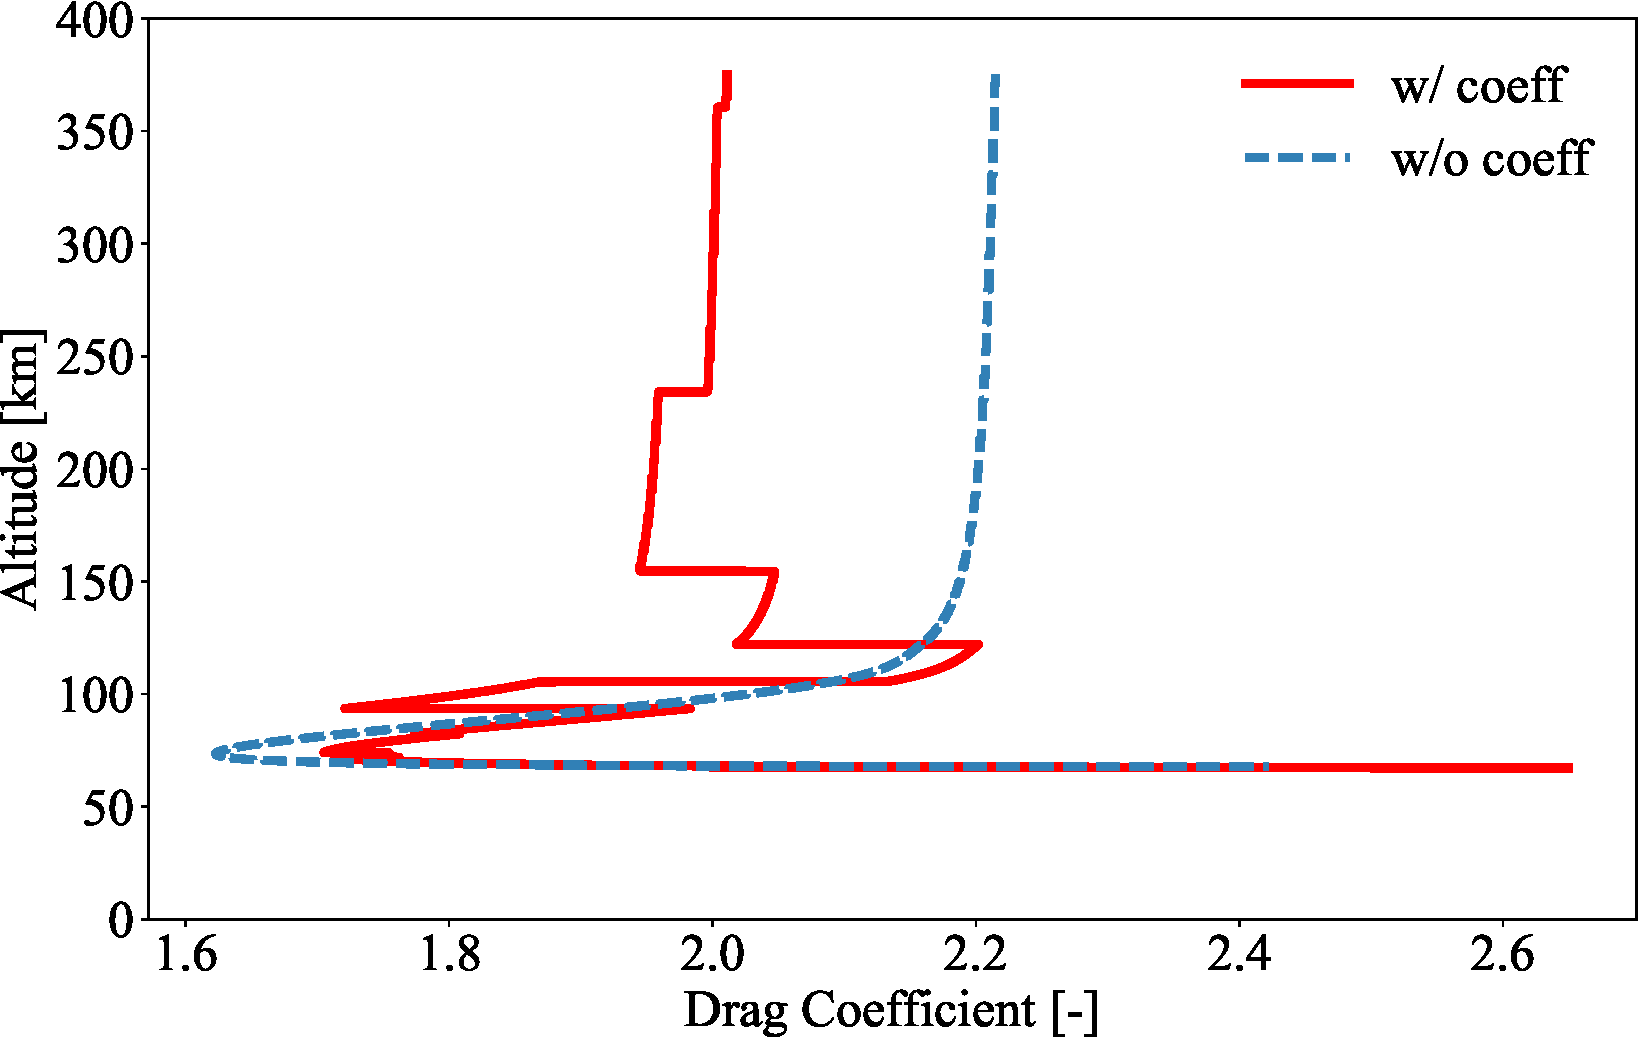
\includegraphics[width=10cm]{fig/couple/cd-coeff/Cd.pdf}
    \caption{抗力係数の補正係数あり(w/)となし(w/o)による抗力係数変化.}
    \label{fig:couble-cd-cd}
\end{figure}
\begin{figure}[H]
    \centering
    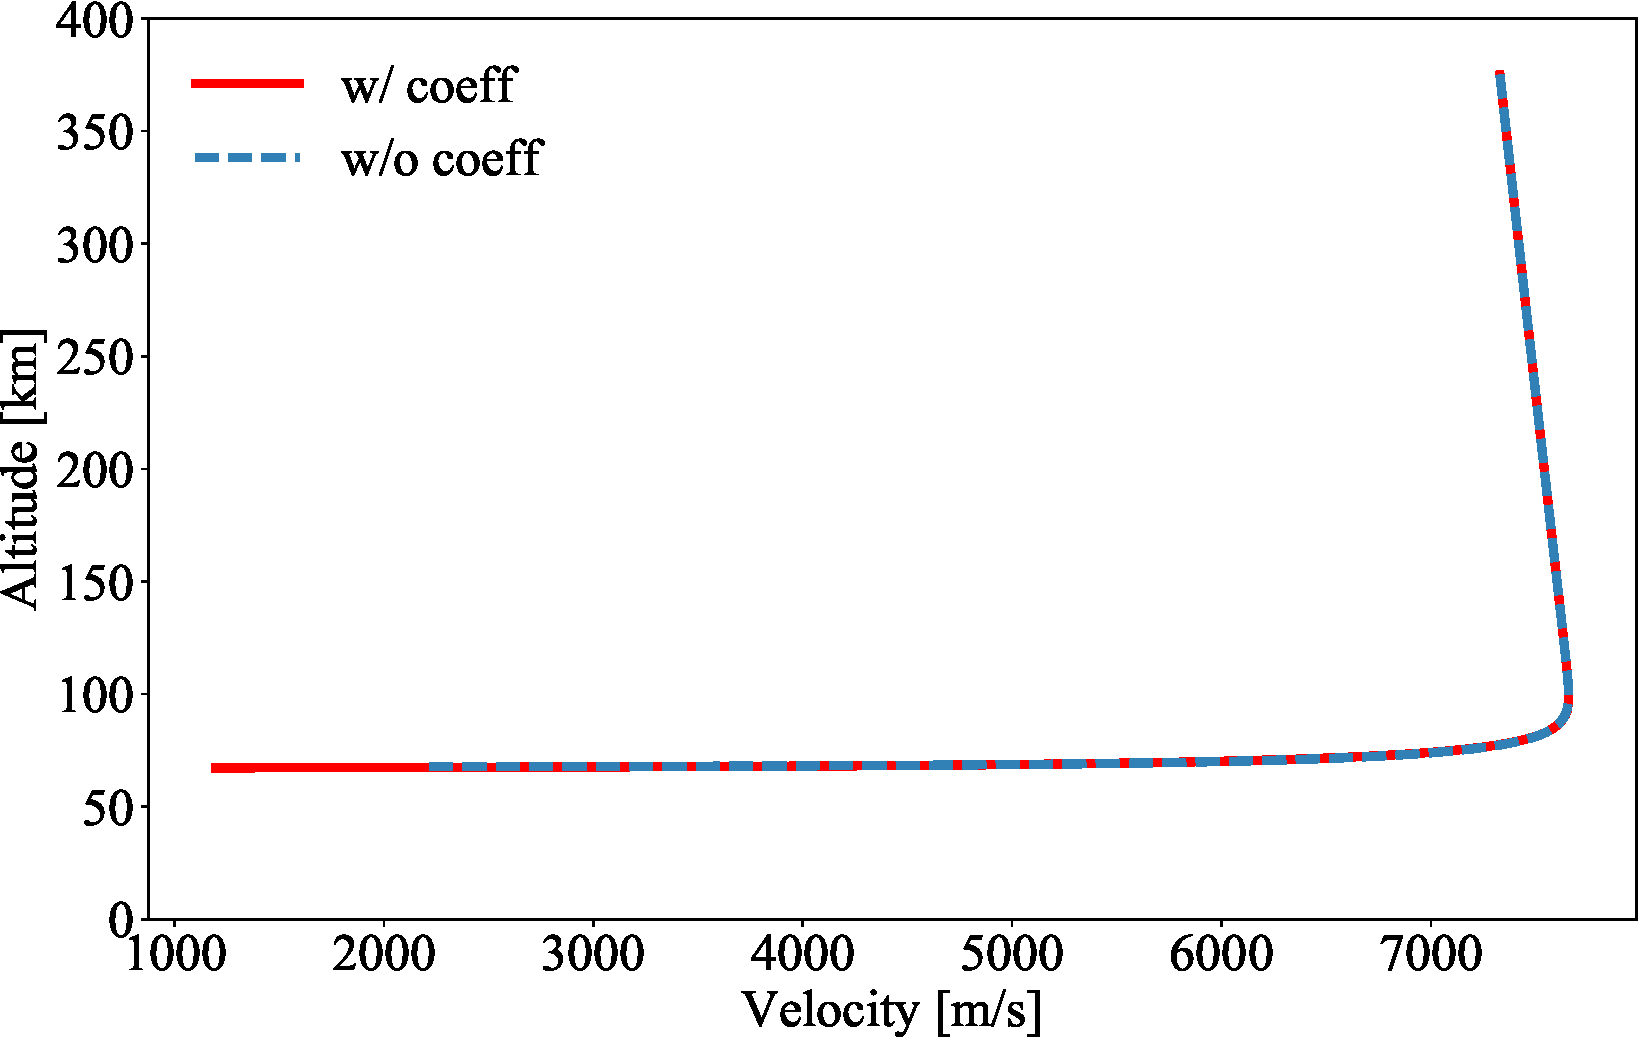
\includegraphics[width=10cm]{fig/couple/cd-coeff/velo.pdf}
    \caption{抗力係数の補正係数あり(w/)となし(w/o)による速度変化.}
    \label{fig:couble-cd-velo}
\end{figure}
\begin{figure}[H]
    \centering
    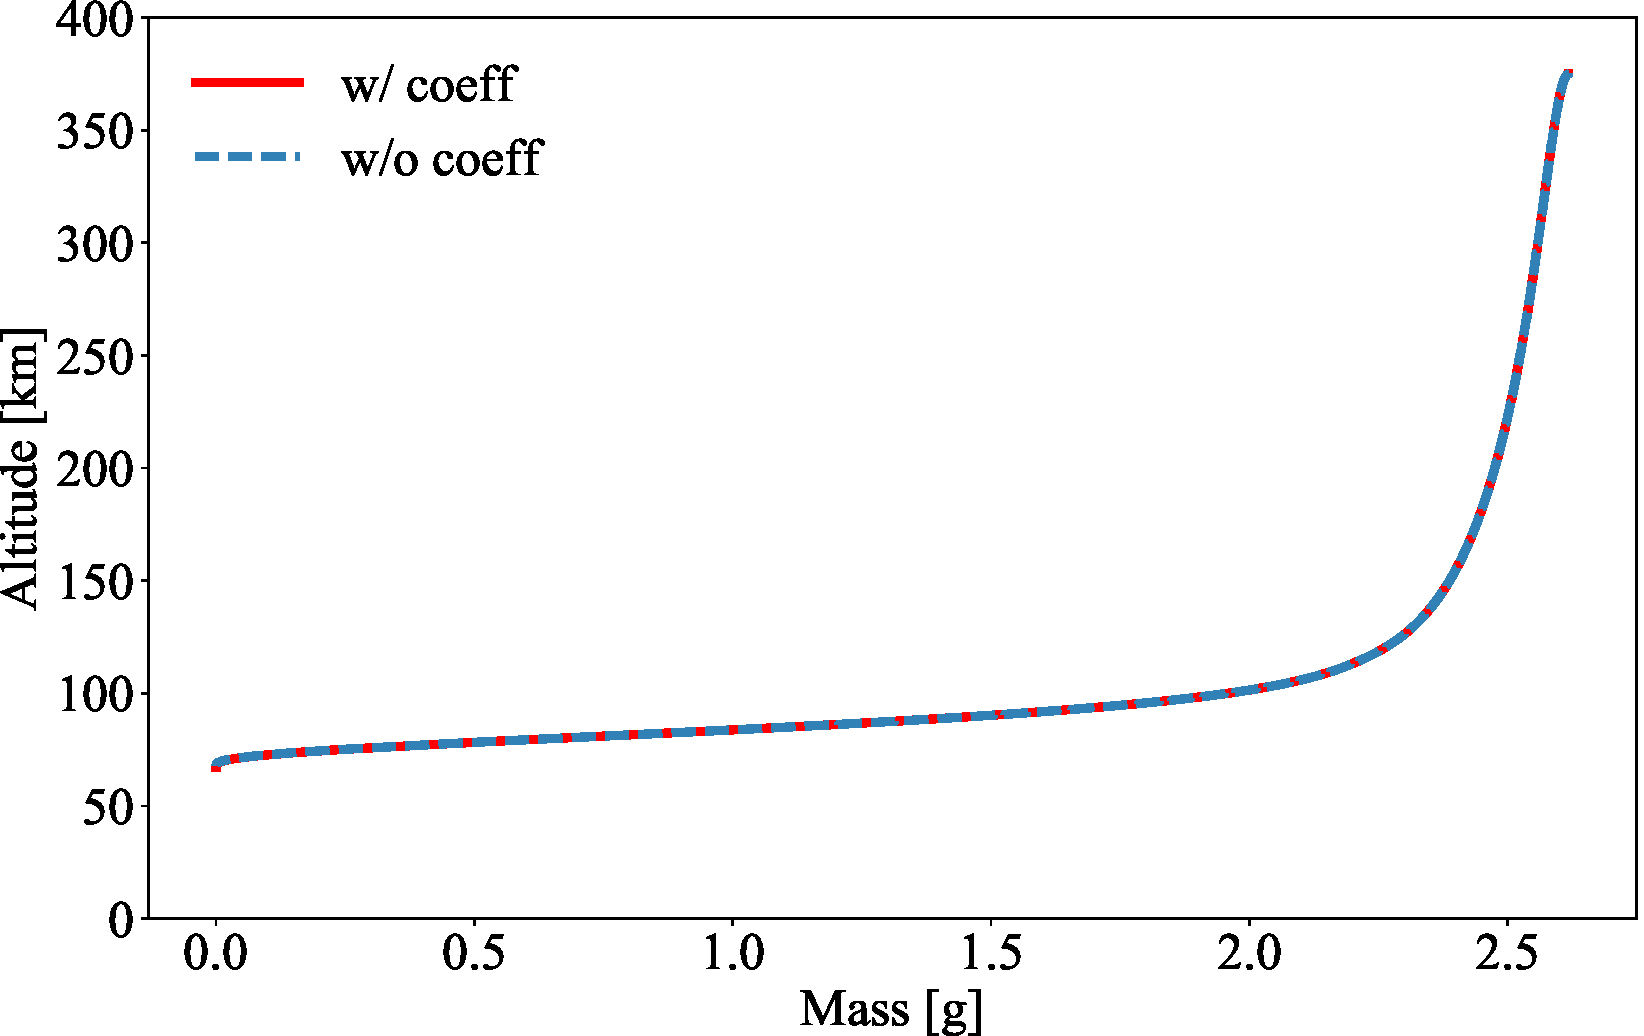
\includegraphics[width=10cm]{fig/couple/cd-coeff/mass.pdf}
    \caption{抗力係数の補正係数あり(w/)となし(w/o)による質量変化.}
    \label{fig:couble-cd-mass}
\end{figure}
\begin{figure}[H]
    \centering
    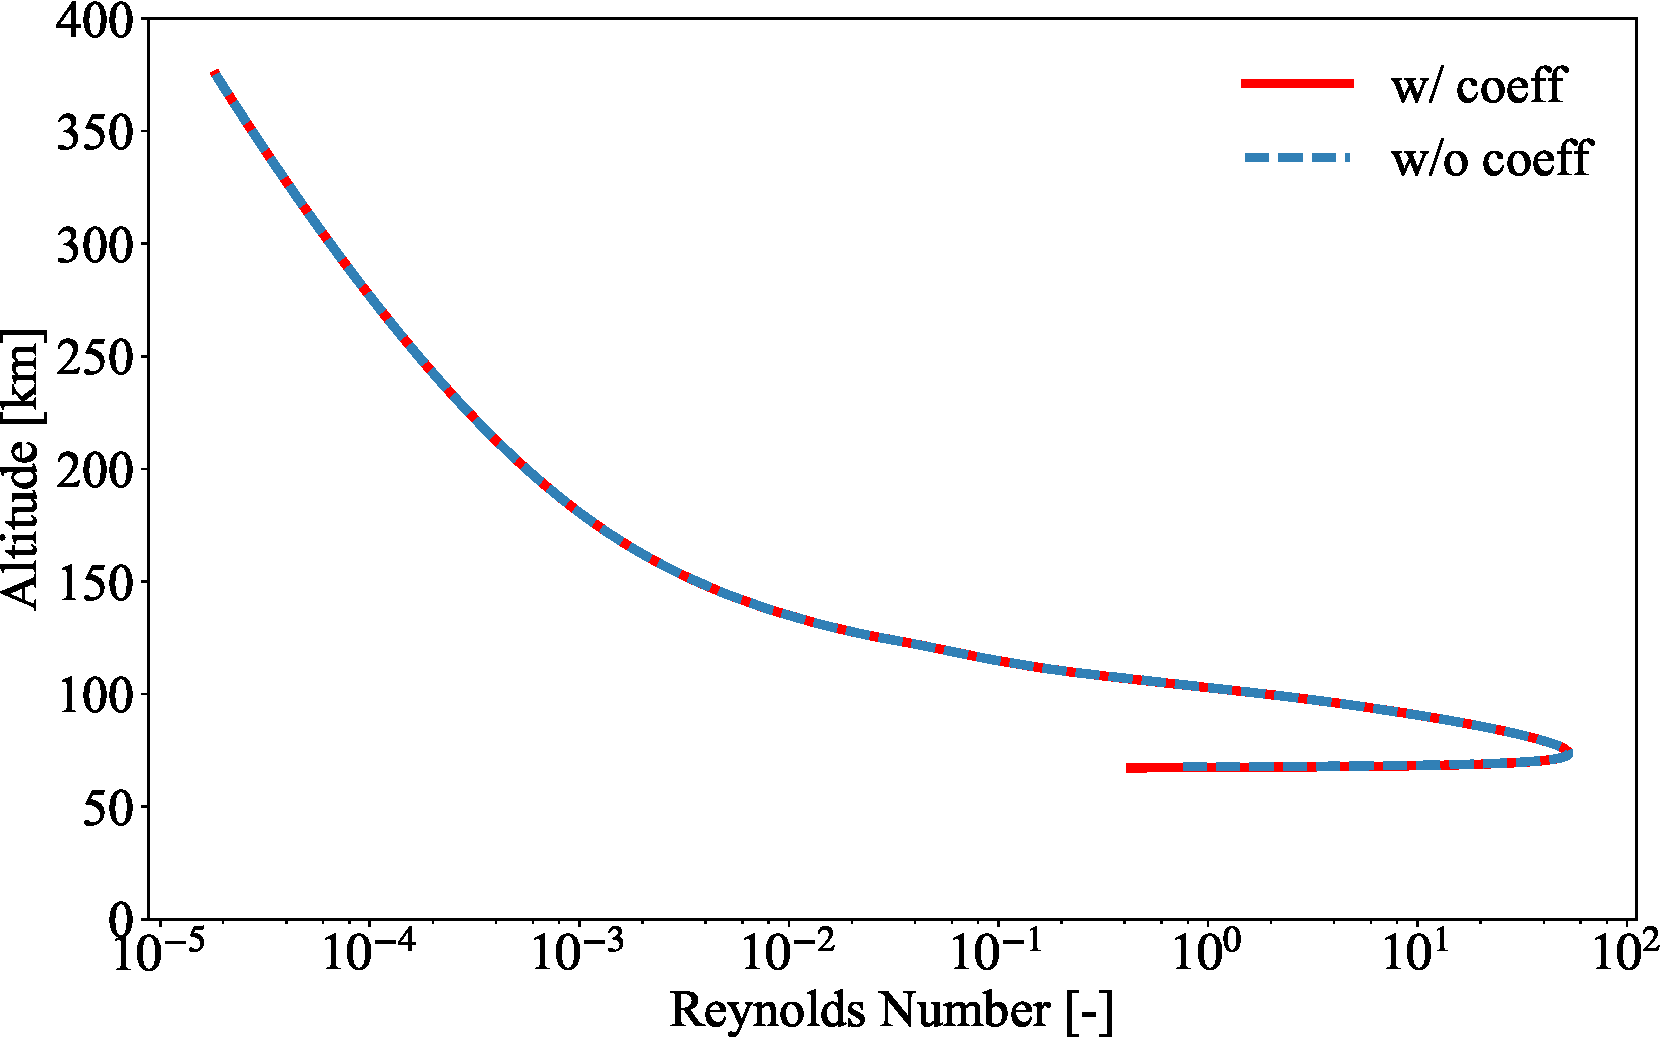
\includegraphics[width=10cm]{fig/couple/cd-coeff/re.pdf}
    \caption{抗力係数の補正係数あり(w/)となし(w/o)によるReynolds数変化.}
    \label{fig:couble-cd-re}
\end{figure}
\begin{figure}[H]
    \centering
    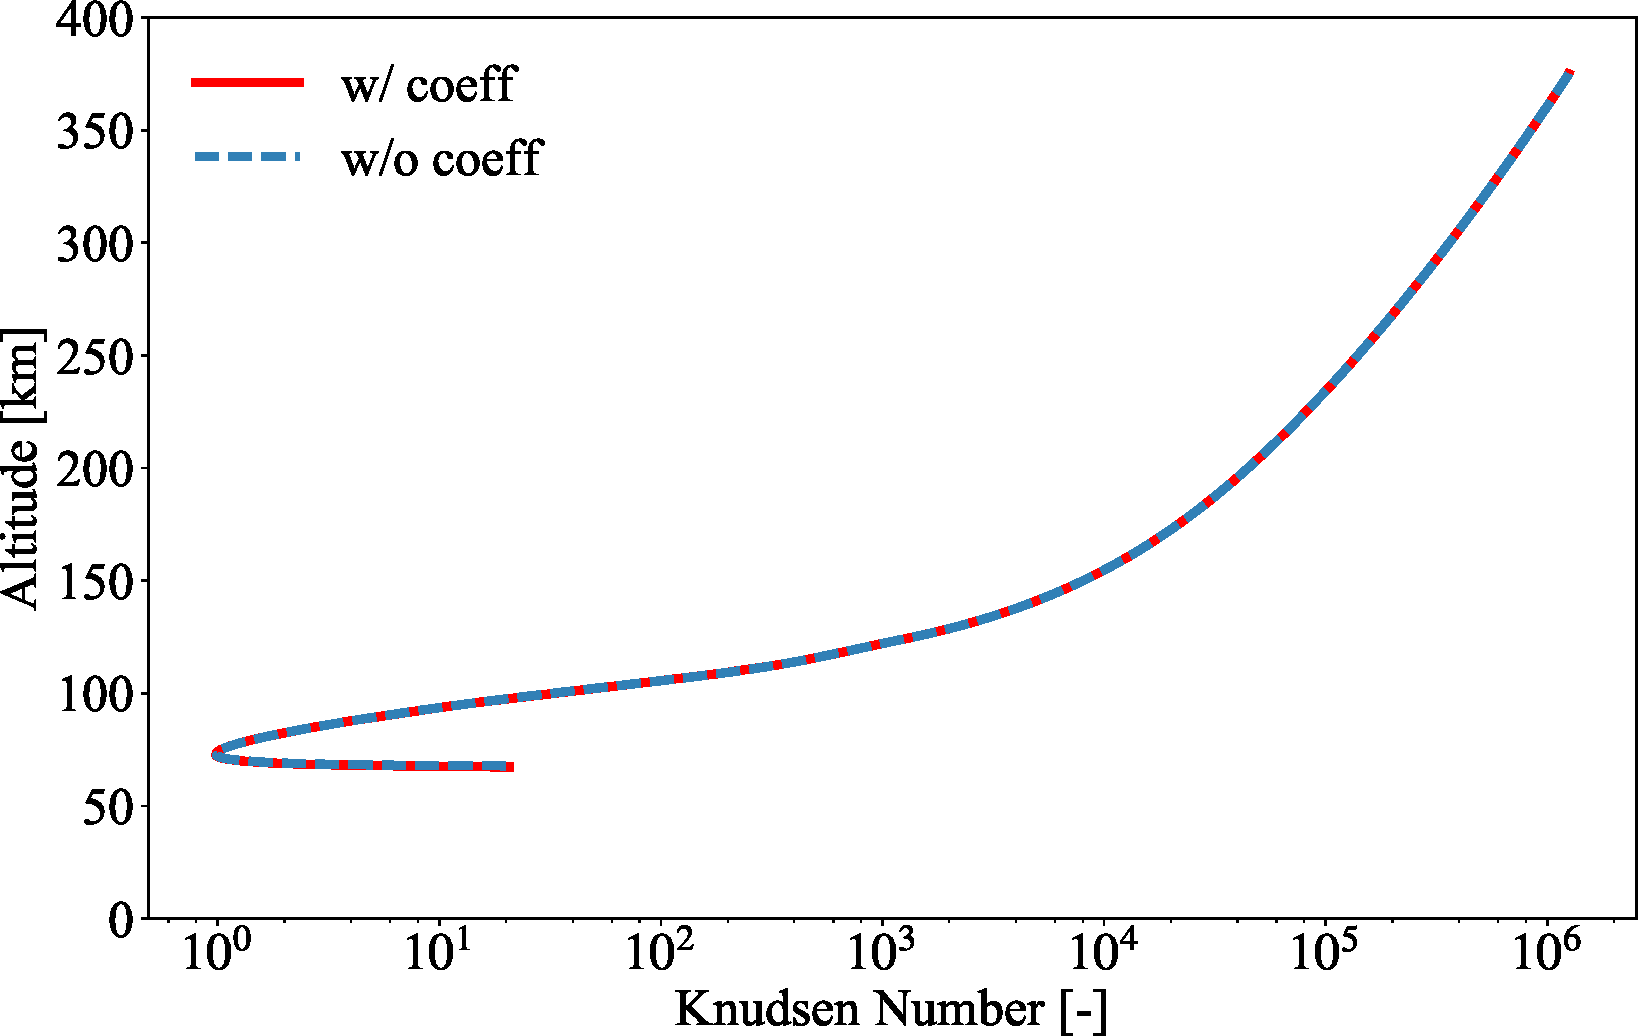
\includegraphics[width=10cm]{fig/couple/cd-coeff/kn.pdf}
    \caption{抗力係数の補正係数あり(w/)となし(w/o)によるKnudsen数変化.}
    \label{fig:couble-cd-kn}
\end{figure}
\begin{figure}[H]
    \centering
    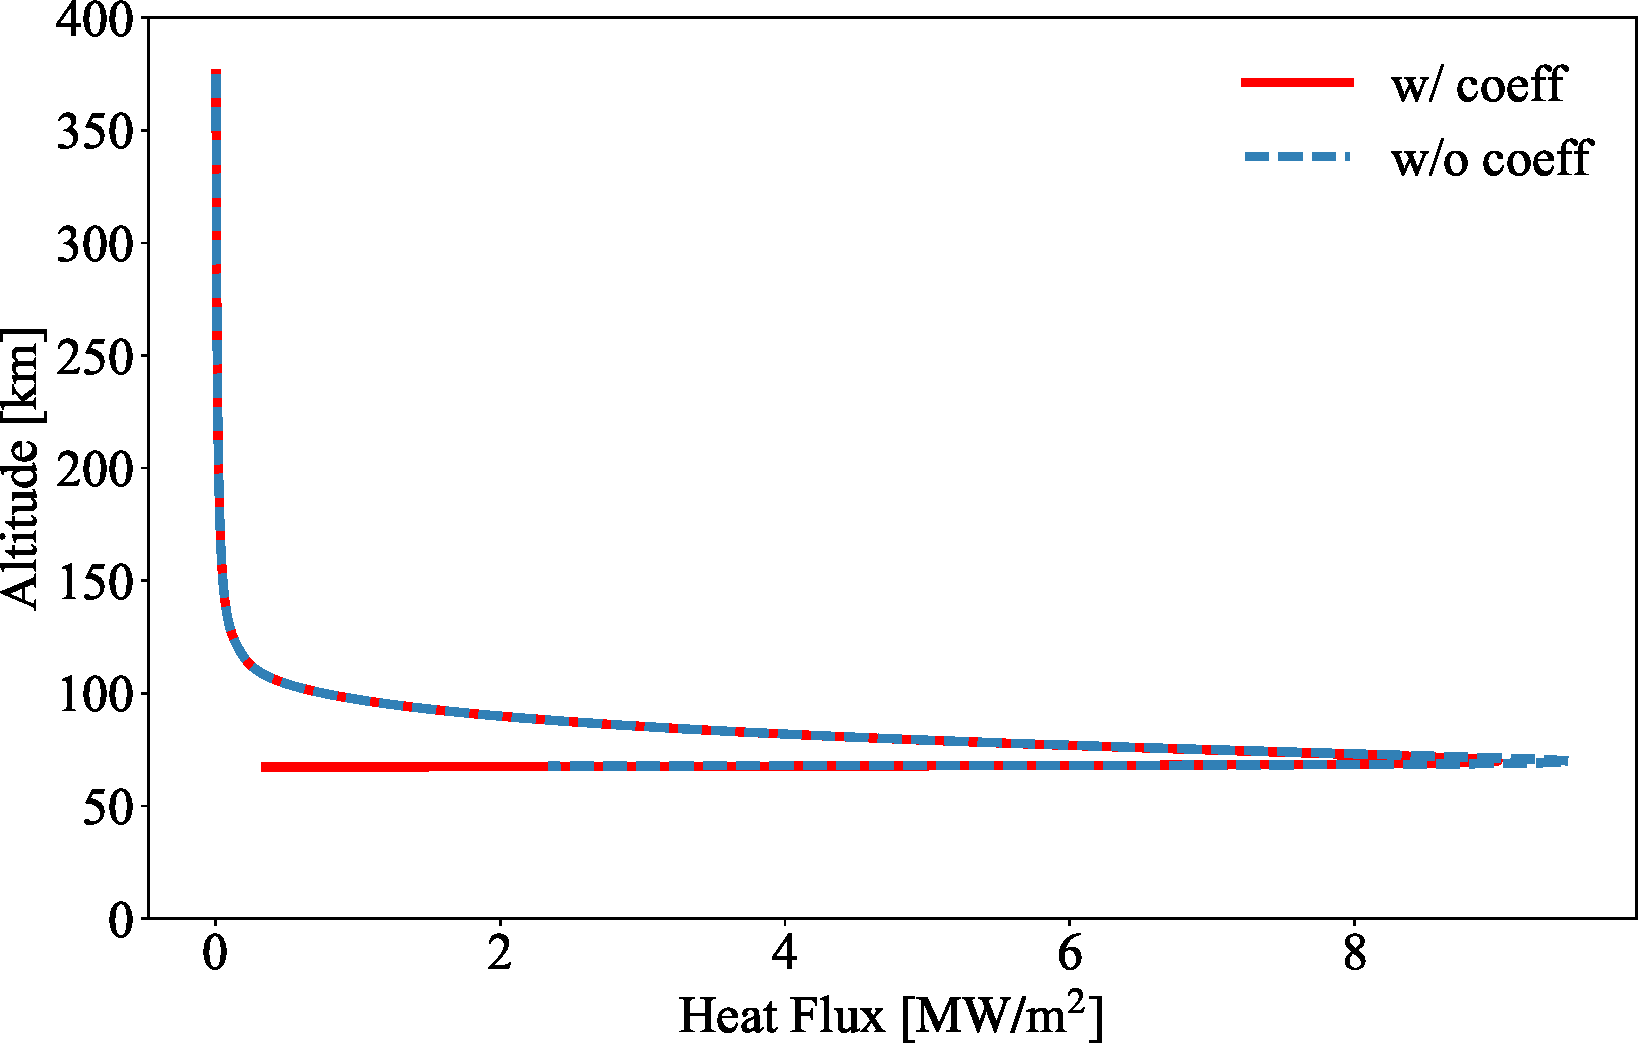
\includegraphics[width=10cm]{fig/couple/cd-coeff/heat.pdf}
    \caption{抗力係数の補正係数あり(w/)となし(w/o)による熱流束変化.}
    \label{fig:couble-cd-heat}
\end{figure}


\section{淀み点熱流束の補正}
\subsection{DSMC法との連成解析による補正係数の算出}
次に,淀み点熱流束について補正を試みる.
DSMC法との連成解析によって得られたKnudsen数に対する淀み点熱流束の補正係数を以下の表に示す.
\begin{table}[H]
\centering
\caption{軌道計算およびDSMC法の連成解析による淀み点熱流束の補正係数}
\begin{tabular}{l|cc}
\hline\hline

$Kn$ & 補正係数($q_0^*$) \\ \hline
\num{1.2d7} &  \num{8.13d-04} \\
\num{1d6  } &  \num{2.41d-03} \\
\num{1d5  } &  \num{2.36d-03} \\
\num{1d4  } &  \num{6.94d-03} \\
\num{1d3  } &  \num{2.59d-02} \\
\num{1d2  } &  \num{7.35d-02} \\
\num{1d1  } &  \num{1.82d-01} \\
\num{2d0  } &  \num{3.66d-01} \\
\num{1d0  } &  \num{4.98d-01} \\
\num{5d-1} &  \num{6.96d-01} \\
\num{2d-1 } &  \num{8.74d-01} \\
\num{1d-1 } &  \num{1.04d0  } \\ \hline\hline
\end{tabular}
\end{table}
ここで,淀み点熱流束の補正係数$q_0^*$の定義は,DSMC法によって得られる淀み点熱流束とDKRモデルによって得られる淀み点熱流束の比であり,以下のように与える.
\begin{equation}
    q_0^* = \dfrac{q_{0,\mathrm{DSMC}}}{q_{0,\mathrm{DKR}}}
\end{equation}

結果を見ると,Knudsen数が大きいほどDKRモデルと乖離し,Knusen数が0.1において概ね一致するということが分かる.
これは,DKRモデルが連続流を仮定しているために自由分子流に近づくほど予測が不正確になるためと考えられる.
さらに,この結果を両対数でプロットし,最小二乗法によって線形近似を行ったものを図~\ref{fig:couble-kn-heat}に示す.
\begin{figure}[H]
    \centering
    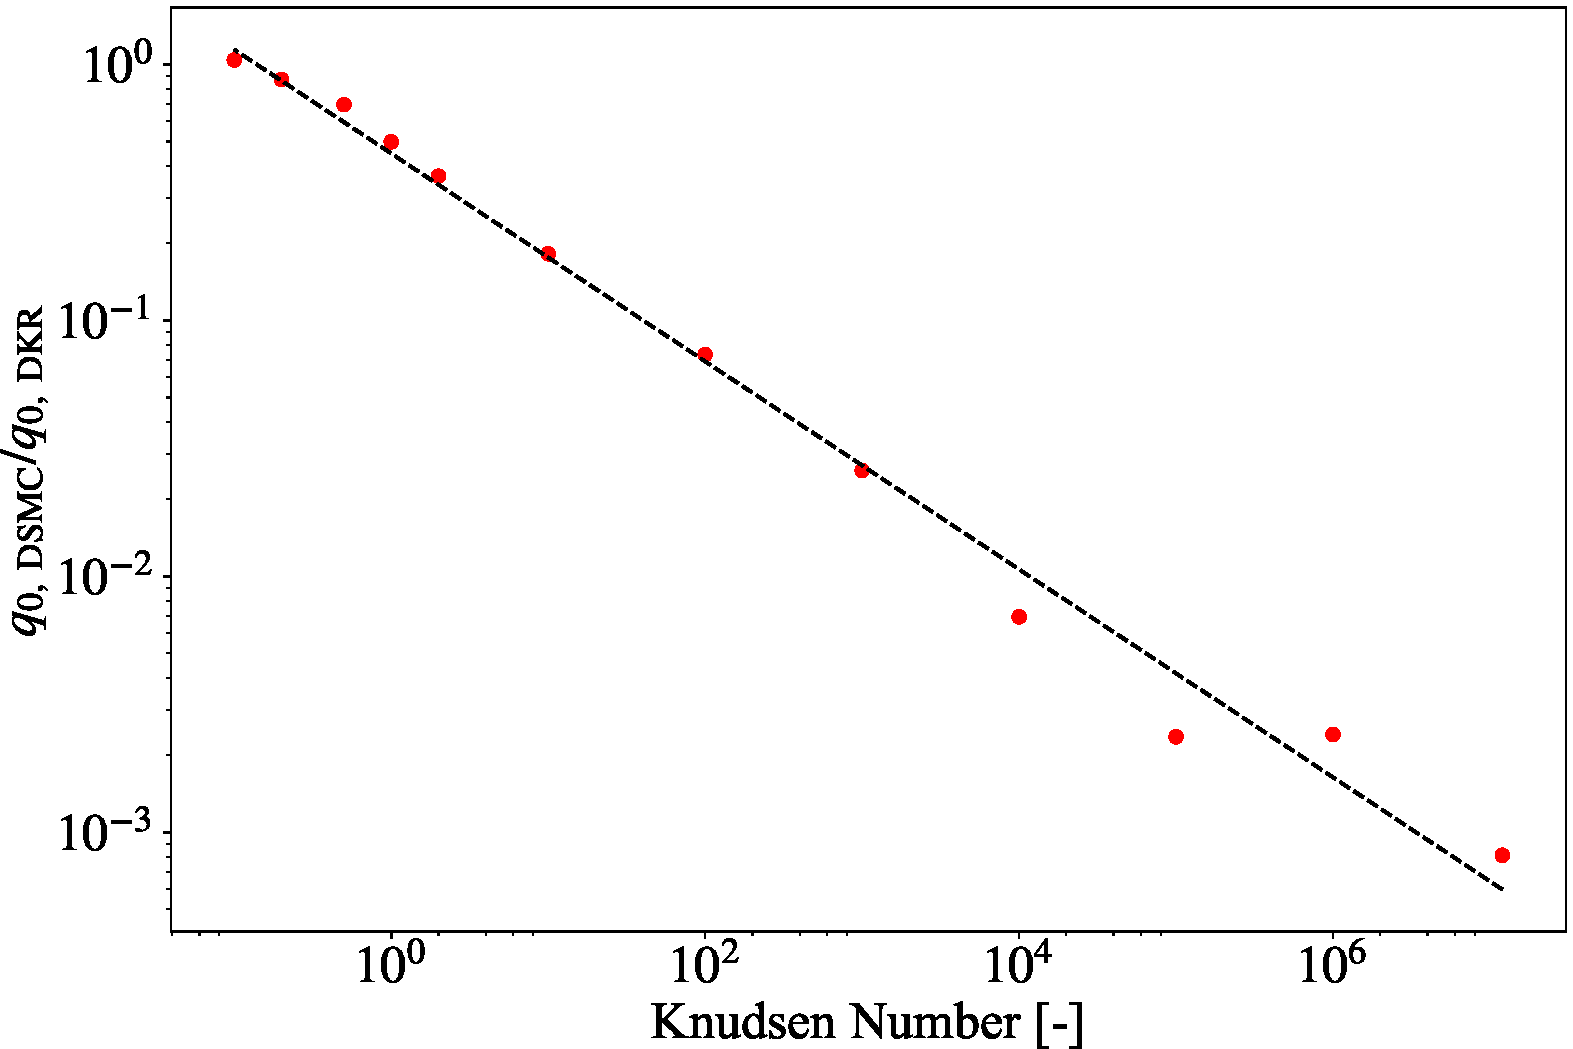
\includegraphics[width=10cm]{fig/couple/kn-heat.pdf}
    \caption{Knudsen数と淀み点熱流束の補正係数の関係(両対数).}
    \label{fig:couble-kn-heat}
\end{figure}
ここで,最小二乗法による傾きは$-0.4062$, 切片は$-0.3481$で相関係数は$-0.9947$となった.
相関係数はほとんど$-1$になっていることからも,Knusen数と補正係数には相関がある.
従って,DKRモデルで得られる淀み点熱流束を以下の式によって補正すればDSMC法での淀み点熱流束に近づく.
\begin{equation}
    q_{0,\mathrm{DKR}}^\prime =
    \begin{cases}
    q_{0,\mathrm{DKR}}\times\exp\left[{-0.4062\times\log_{10}\left({Kn}-0.3481\right)}\right], & Kn > 0.1, \\
    q_{0,\mathrm{DKR}}, & Kn \le 0.1.
    \end{cases}
\end{equation}
ただし,$q_{0,\mathrm{DKR}}^\prime$は補正後の淀み点熱流束を示す.


\subsection{淀み点熱流束への補正による軌道への影響}
次に,この補正を行った場合と行わない場合の軌道計算の比較を行う.
ただし,抗力係数に関しては,先に述べたとおり補正による影響は無視できるほど小さく,
Hendersonのモデル式に従うものとした.

淀み点熱流束への補正あり・なしの速度変化および質量変化を図~\ref{fig:couble-heat-velo},図~\ref{fig:couble-heat-mass}に示す.
速度変化を見ると,両者は概ね一致している.
しかし,質量変化を見ると,補正を加えることによって特に高高度での質量減少が非活性になっている.
さらに,高度を落として連続流に近づくと,高度80~km付近で急激に質量が減少し,補正を加えない場合とほとんど同じ高度で消滅していることが分かる.

次に,補正あり・なしでの淀み点熱流束変化を図~\ref{fig:couble-heat-heat}に示す.
補正を加えた場合,極大値が約1.4倍に増大したことが確認できる.
しかし,極大値を迎える高度より高高度では補正を加えた方が小さくなっており,
高度80~km付近で両者が交差している.

また,淀み点熱流束への補正あり・なしでの抗力係数変化・Mach数変化・Reynolds数変化・Knudsen数変化を
それぞれ図~\ref{fig:couble-heat-cd}から図~\ref{fig:couble-heat-kn}に示す.
それぞれ極大値・極小値の多少の差異が見られるが,概ね両者は一致している.

さらに,淀み点熱流束に補正を加えた場合の最大発光地点を比較する.
ただし,人工衛星からの放出角度が不明なため,初期座標からの変化角にその高度における地球中心からの距離をかけ合わせた,周方向距離で議論する.
補正を加えない場合の最大発光地点は周方向に6413~kmで,
補正を加えた場合は6464~kmであった.
両者の差異は51~kmであり,
ALE人工衛星は発光地点から半径200~km以内で地上から観測されるとしており~\cite{ALECoLtd30:online},
想定される観測範囲から考えるとこの差異は許容できるものではないと考えられる.


また,得られた軌道計算結果において,流星源が消滅するタイミングに差異が現れていることが分布から確認できる.
これは消滅と判断する閾値の違いである.
第\ref{chap:trajectory}章で述べたように,質量がマシンゼロになるまでの議論は必要ないため,\SI{1e-9}{g}で計算を終了している.
しかし,補正を加えた場合では数値的な振動が発生したため,消滅の閾値を\SI{1e-7}{g}に更新している.
この更新によって消滅のタイミングが変化した.
閾値の変更については,微小質量であることに加え,発光にはほとんど寄与しないため許容できる.

以上の結果により,DKRモデルをそのまま使用した場合と,
DSMC法との連成解析によって補正を加えた場合での軌道計算結果は大きく異なり,
特に高度100~km以上の高高度における質量減少の振る舞いに差異が生じることが分かった.
また,最大発光地点を比較するとその差異は51~kmであり,観測に与える影響は大きいことが分かった.

\begin{figure}[H]
    \centering
    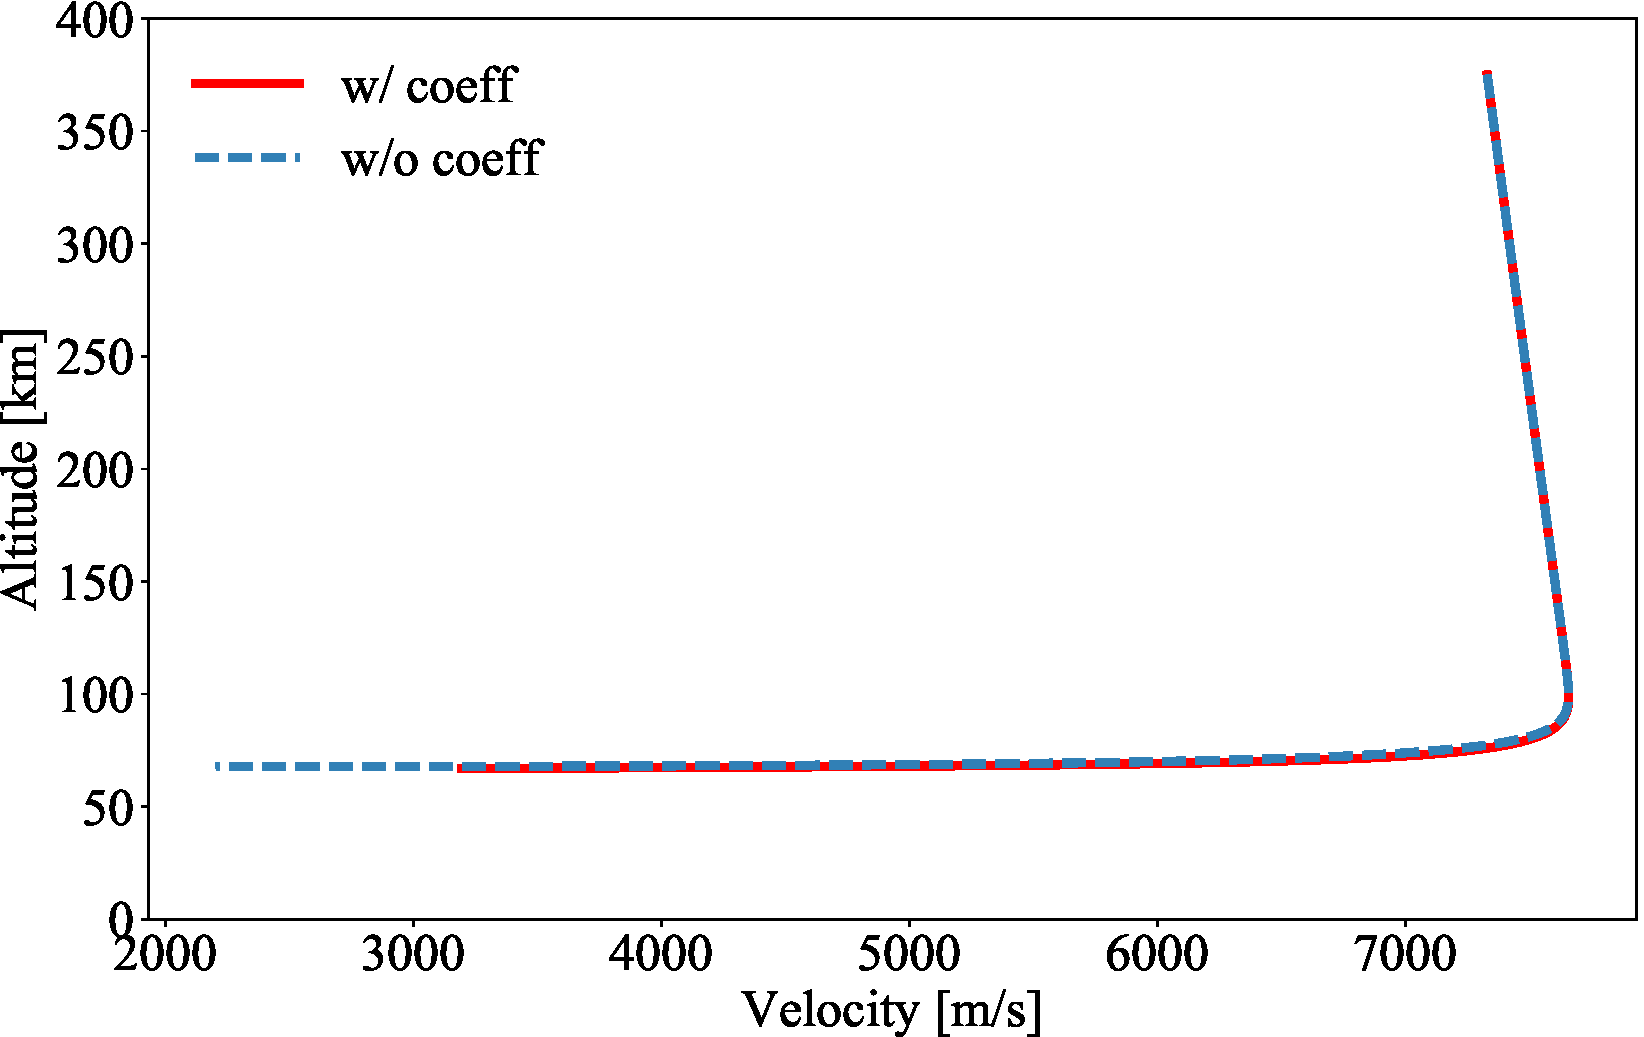
\includegraphics[width=10cm]{fig/couple/heat-coeff/velo.pdf}
    \caption{淀み点熱流束の補正係数あり(w/)となし(w/o)による速度変化.}
    \label{fig:couble-heat-velo}
\end{figure}
\begin{figure}[H]
    \centering
    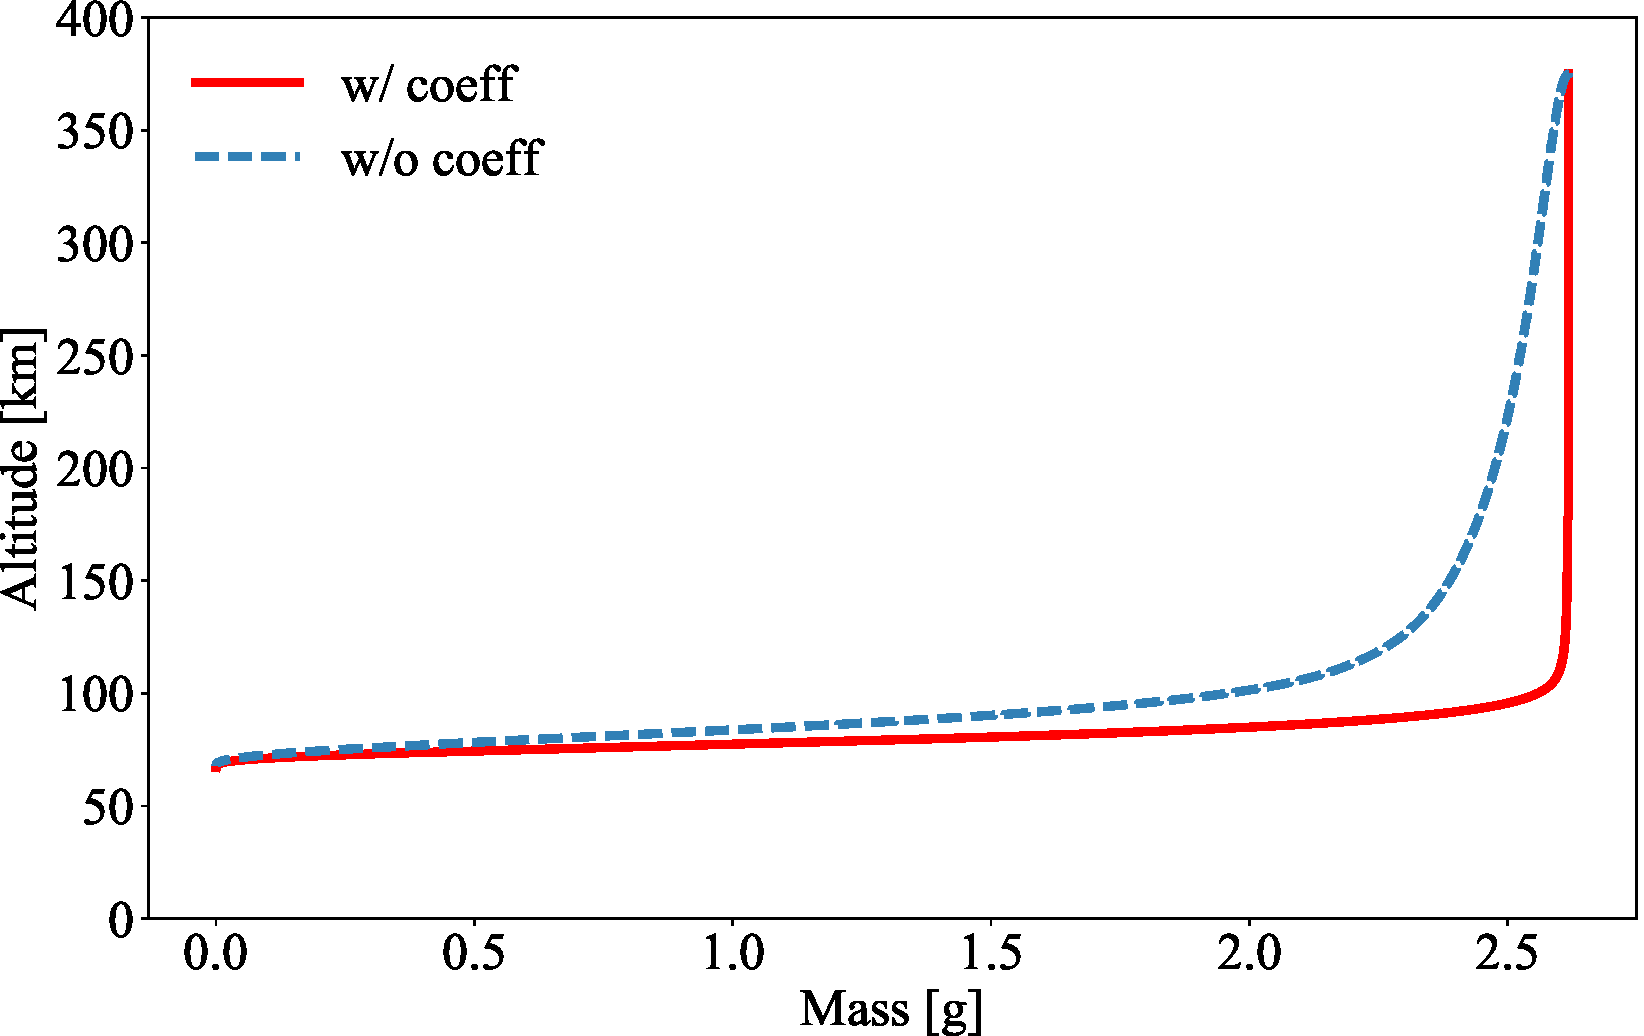
\includegraphics[width=10cm]{fig/couple/heat-coeff/mass.pdf}
    \caption{淀み点熱流束の補正係数あり(w/)となし(w/o)による質量変化.}
    \label{fig:couble-heat-mass}
\end{figure}
\begin{figure}[H]
    \centering
    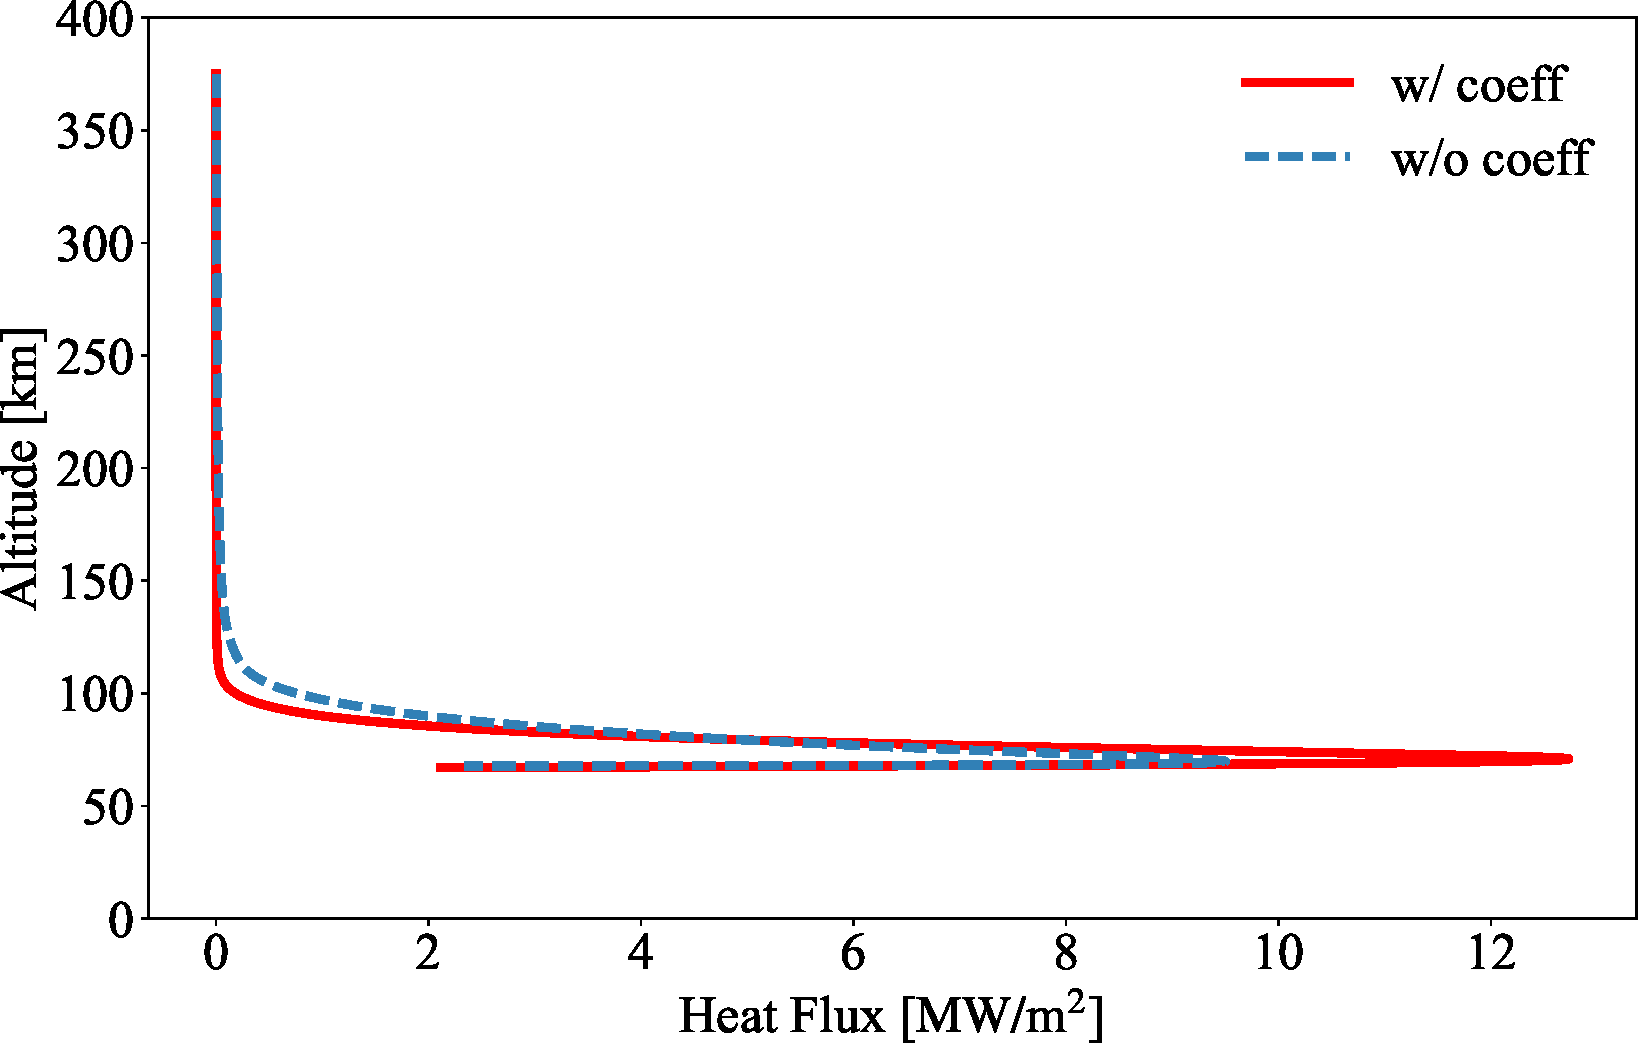
\includegraphics[width=10cm]{fig/couple/heat-coeff/heat.pdf}
    \caption{補正係数あり(w/)となし(w/o)による淀み点熱流束変化.}
    \label{fig:couble-heat-heat}
\end{figure}
\begin{figure}[H]
    \centering
    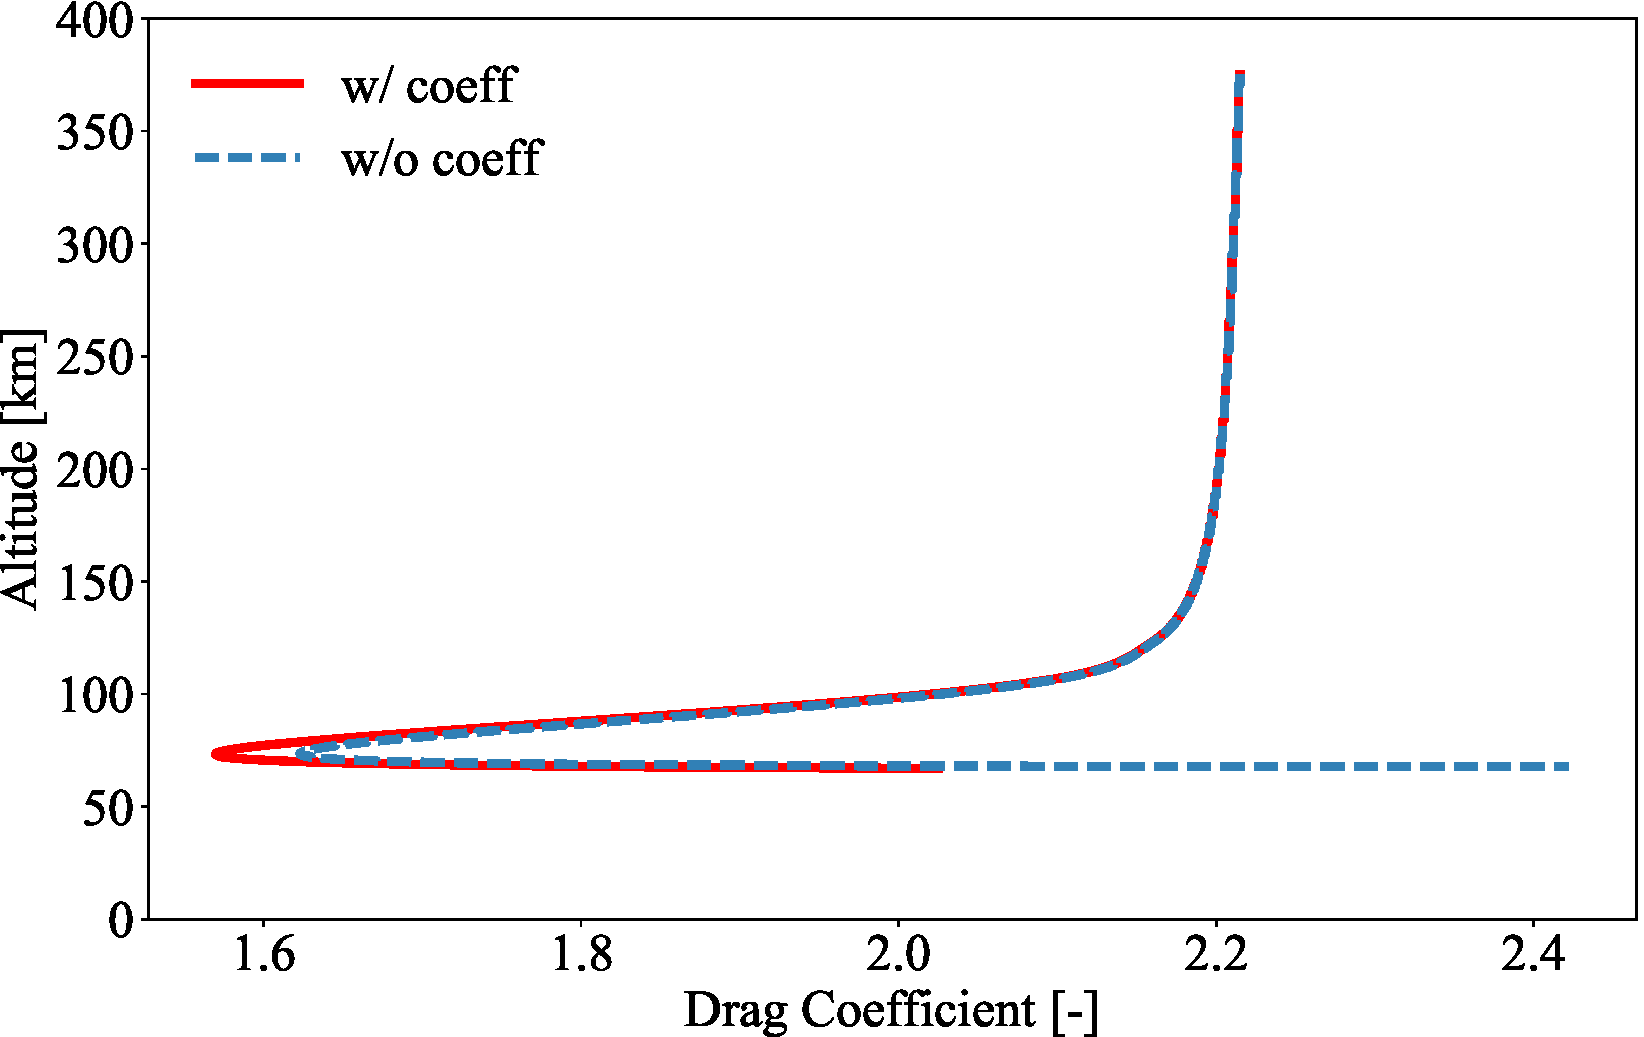
\includegraphics[width=10cm]{fig/couple/heat-coeff/cd.pdf}
    \caption{淀み点熱流束の補正係数あり(w/)となし(w/o)による抗力係数変化.}
    \label{fig:couble-heat-cd}
\end{figure}
\begin{figure}[H]
    \centering
    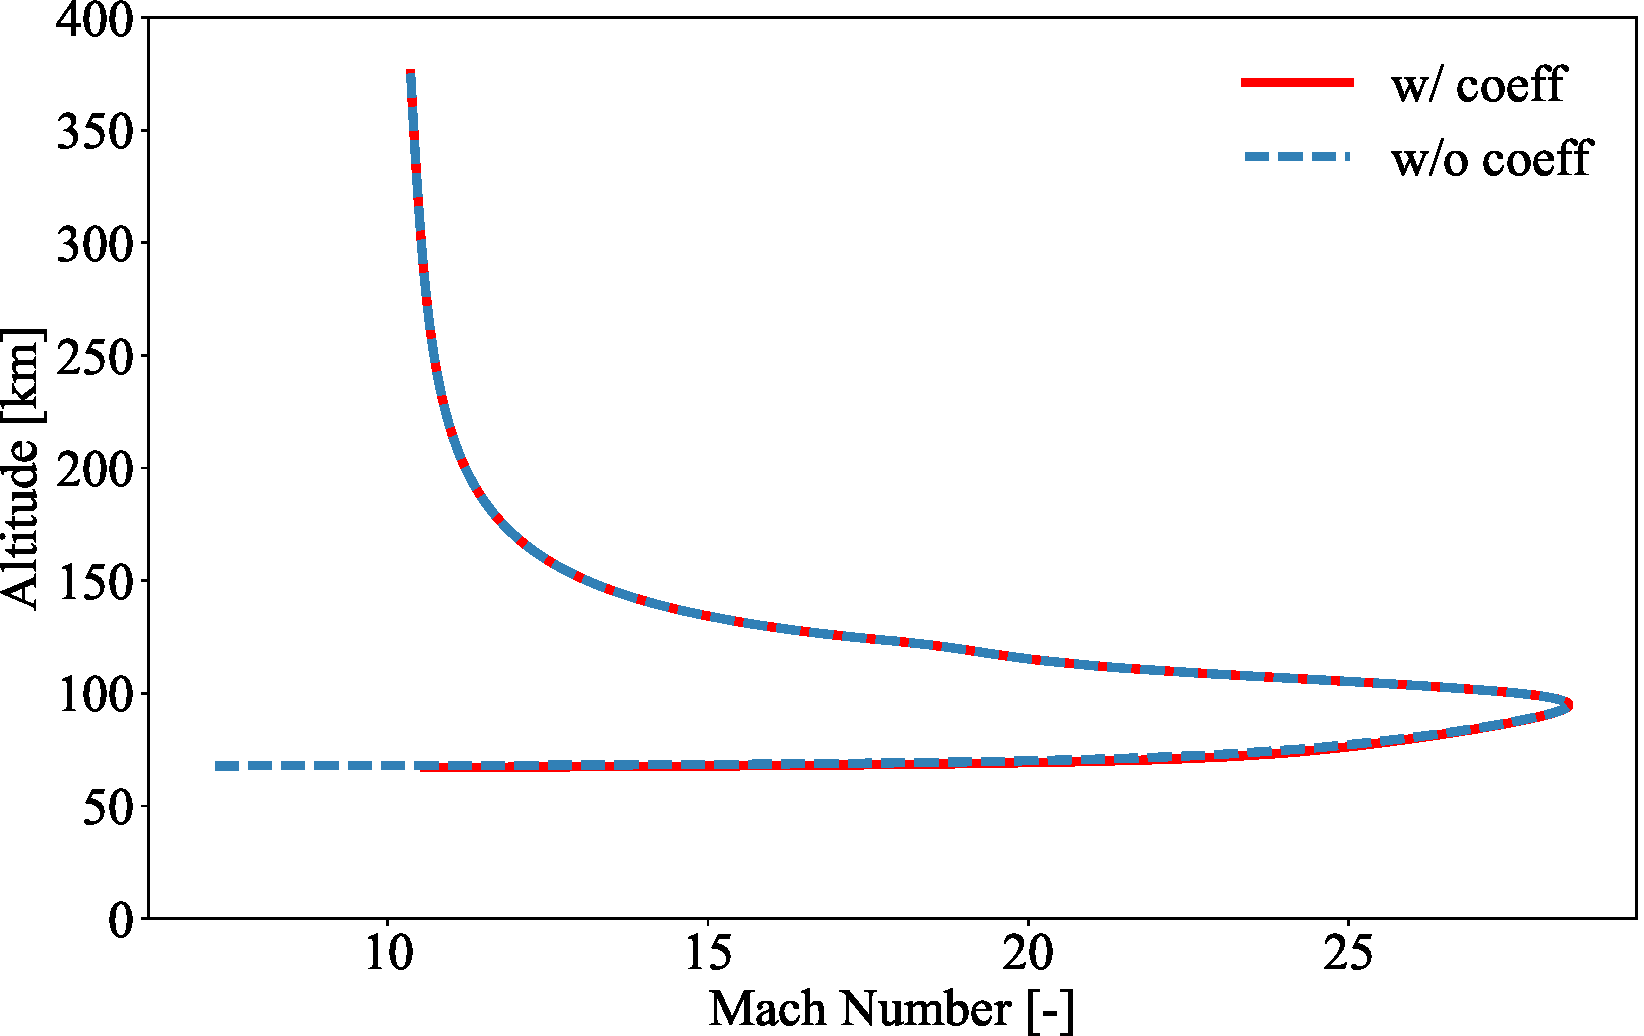
\includegraphics[width=10cm]{fig/couple/heat-coeff/mach.pdf}
    \caption{淀み点熱流束の補正係数あり(w/)となし(w/o)によるMach数変化.}
    \label{fig:couble-heat-mach}
\end{figure}
\begin{figure}[H]
    \centering
    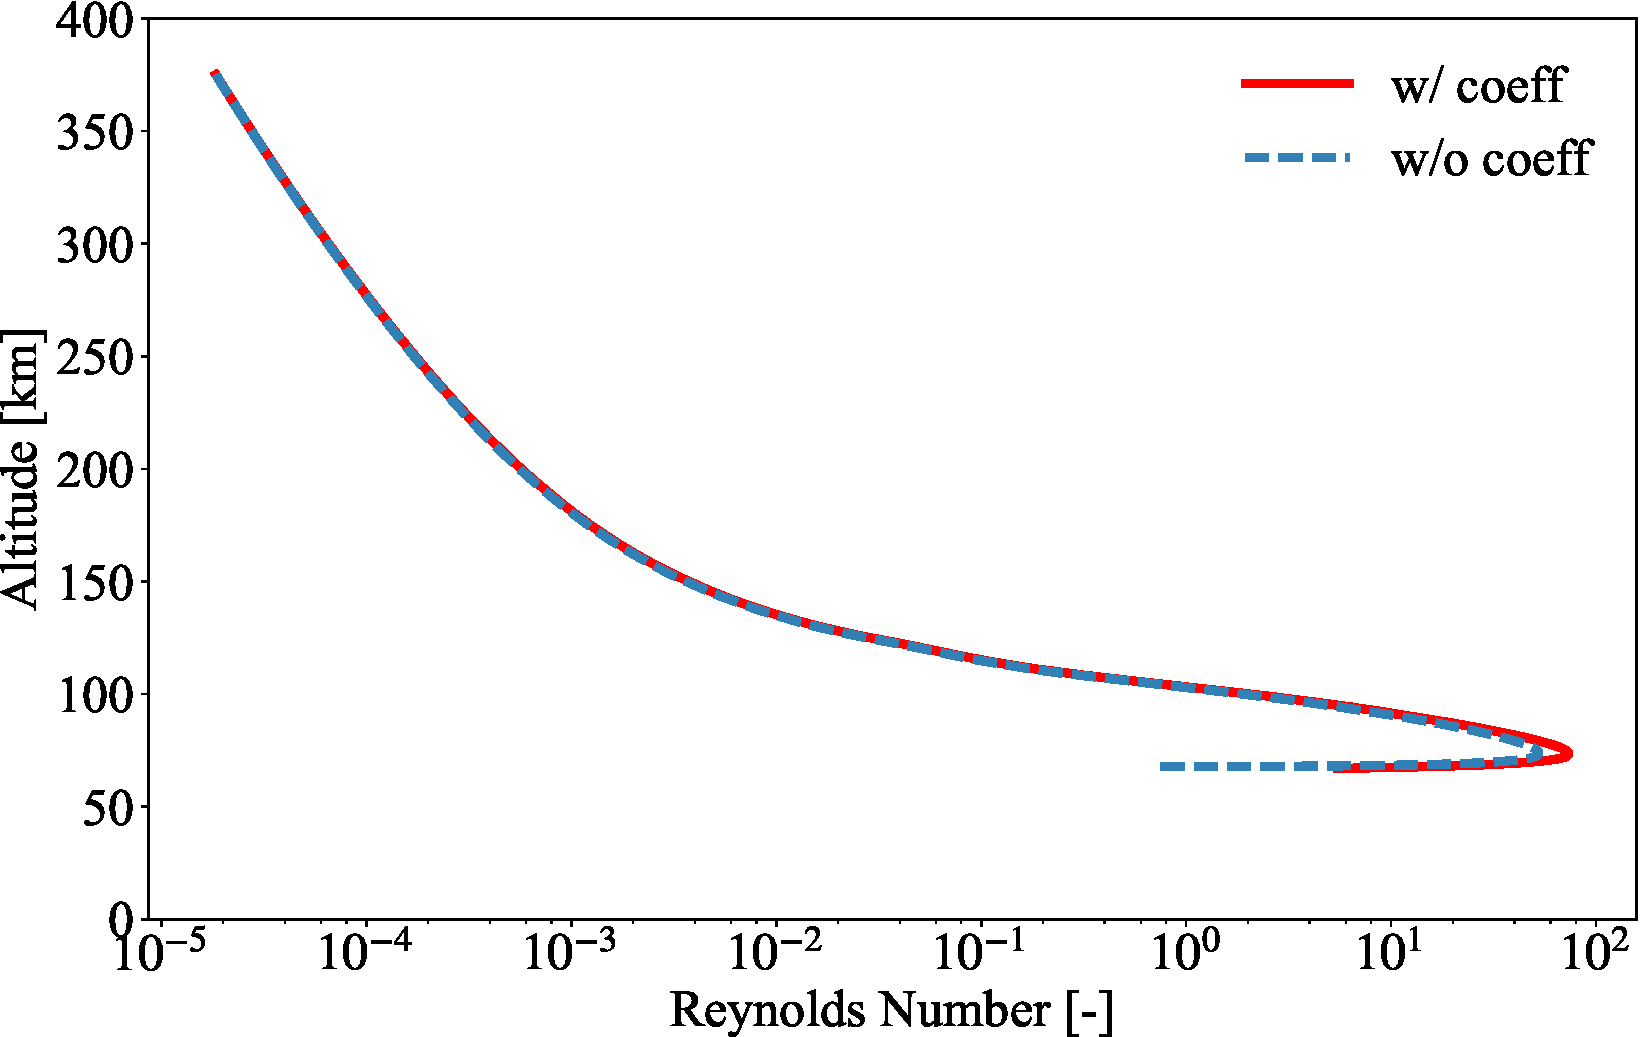
\includegraphics[width=10cm]{fig/couple/heat-coeff/re.pdf}
    \caption{淀み点熱流束の補正係数あり(w/)となし(w/o)によるReynolds数変化.}
    \label{fig:couble-heat-re}
\end{figure}
\begin{figure}[H]
    \centering
    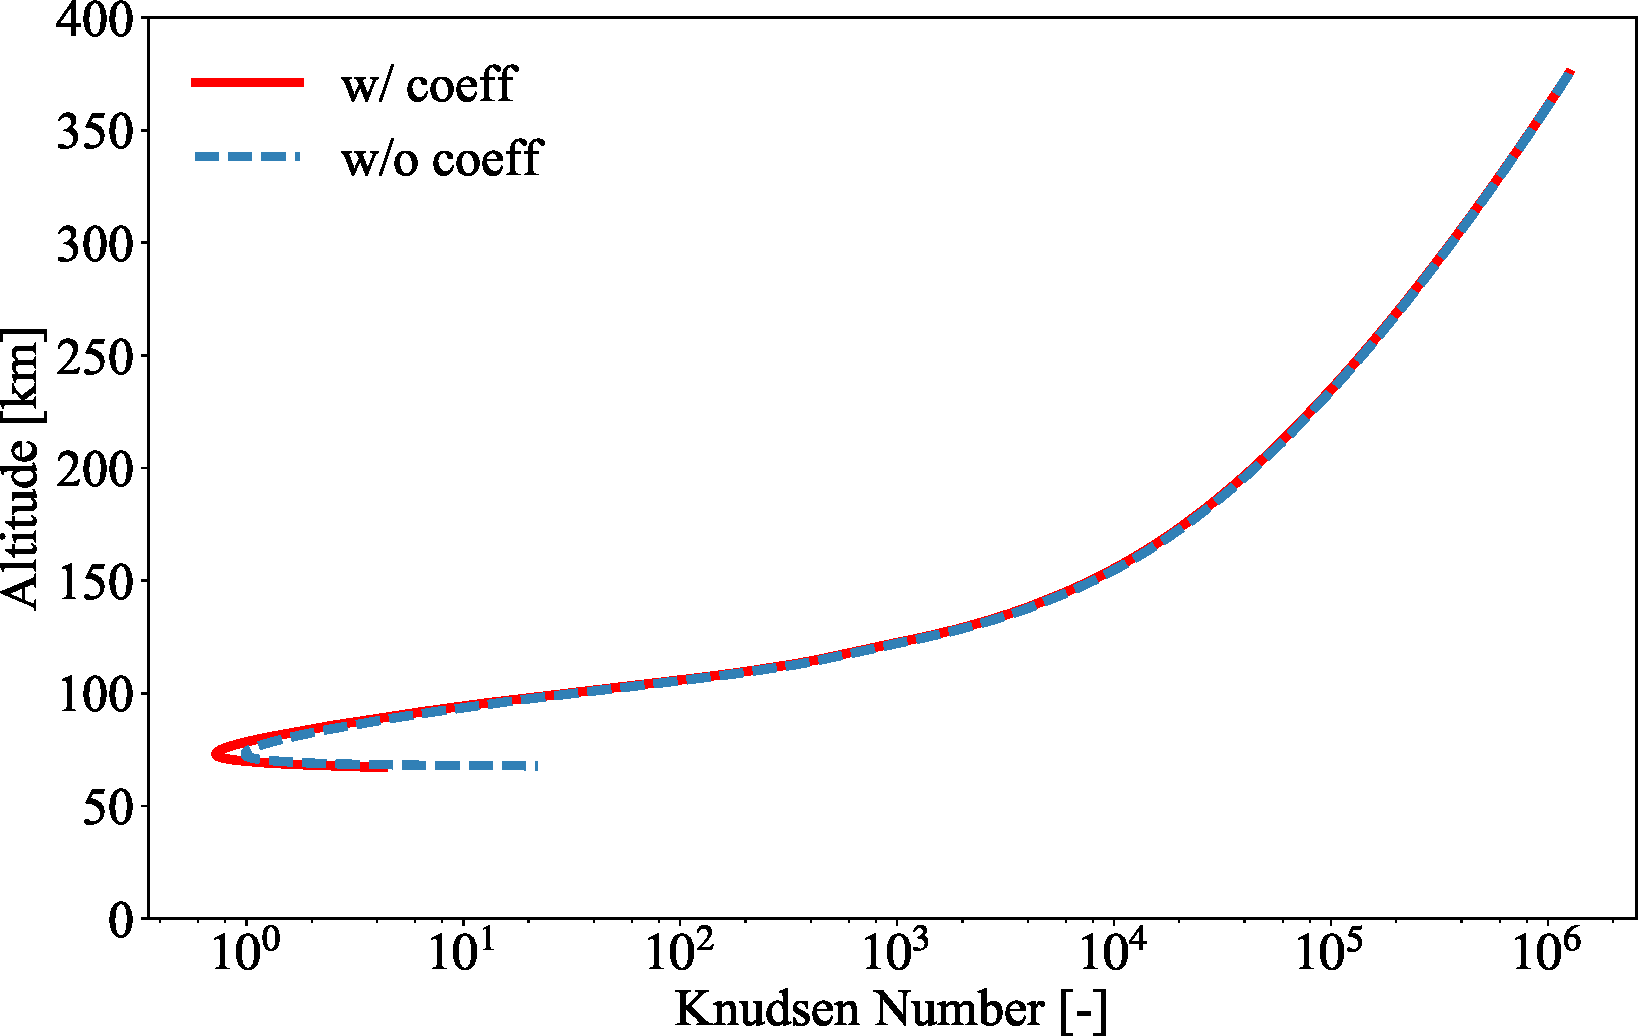
\includegraphics[width=10cm]{fig/couple/heat-coeff/kn.pdf}
    \caption{淀み点熱流束の補正係数あり(w/)となし(w/o)によるKnudsen数変化.}
    \label{fig:couble-heat-kn}
\end{figure}